\begin{figure}[t]
  \usetikzlibrary{decorations.pathreplacing}

\definecolor{tak}{HTML}{d3e2ff}
\definecolor{vol}{HTML}{deffb0}
\definecolor{leeg}{HTML}{ffc5b7}

\hspace{0.055\textwidth}
\begin{adjustbox}{minipage=\textwidth, scale=0.65}
  \centering
\begin{tikzpicture}

\node[inner sep=0pt] (level_0) at (0.0cm,16.5cm)
    {
\includegraphics[width=5cm]{./img/raw/hs-octree-layers/0.png}};
\node[inner sep=0pt] (level_0) at (0.0cm,11cm)
    {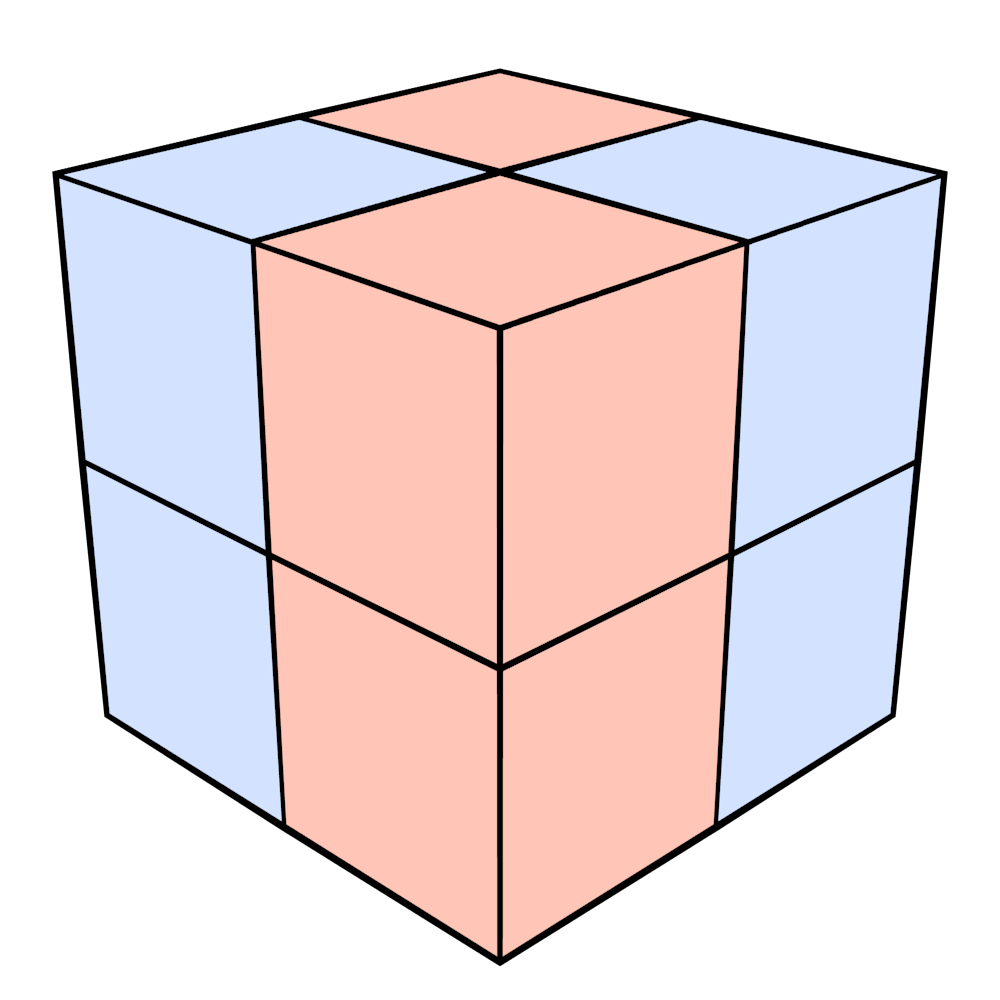
\includegraphics[width=5cm]{./img/raw/hs-octree-layers/1.png}};
\node[inner sep=0pt] (level_0) at (0.0cm,5.5cm)
    {
\includegraphics[width=5cm]{./img/raw/hs-octree-layers/2.png}};
\node[inner sep=0pt] (level_3) at (0.0cm, 0.0cm)
    {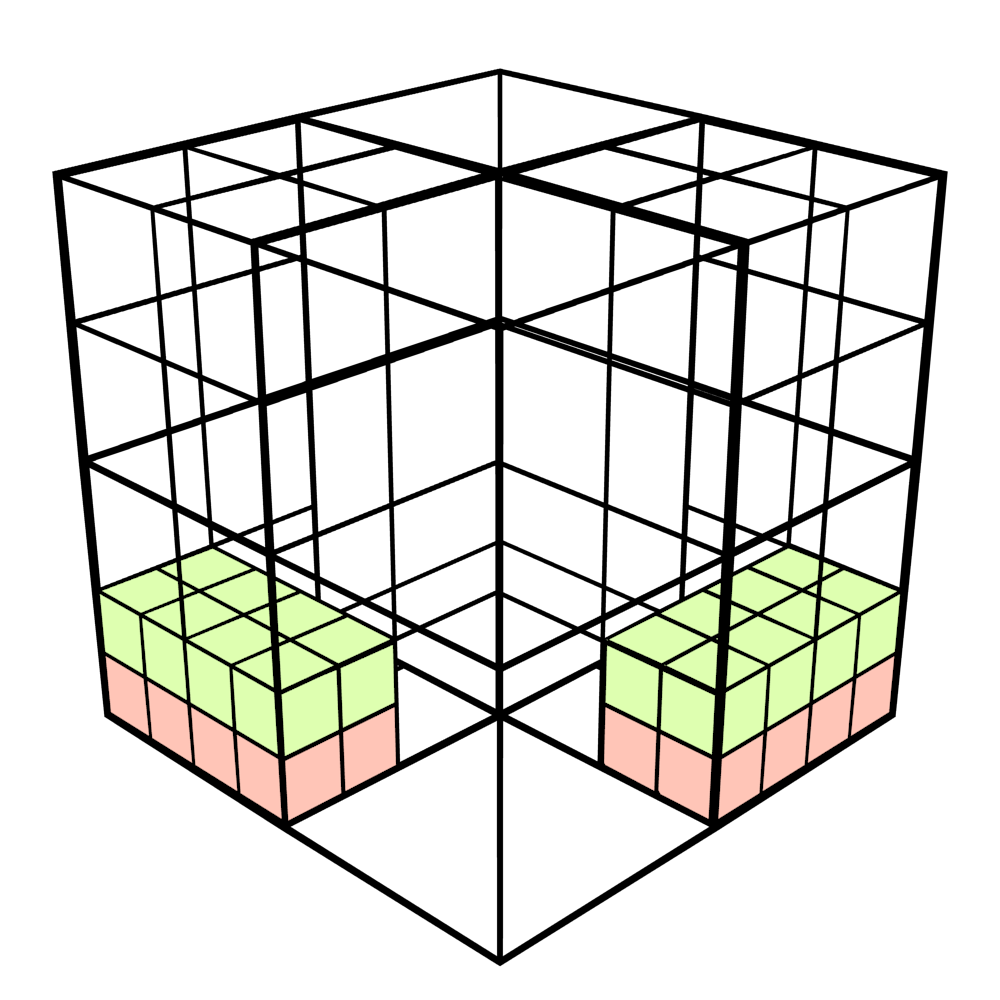
\includegraphics[width=5cm]{./img/raw/hs-octree-layers/3.png}};


\node (i1) at (0cm, 14.25cm) {};
\node (i2) at (0cm, 13.25cm) {};
\node (i3) at (0cm, 8.75cm) {};
\node (i4) at (0, 7.75cm) {};
\node (i5) at (0, 3.25cm) {};
\node (i6) at (0, 2.25cm) {};

\draw[-latex]  (i1) -> (i2);
\draw[-latex]  (i3) -> (i4);
\draw[-latex]  (i5) -> (i6);

\node (l1) at (-2.cm, 18.75cm) {Laag 0};
\node (l1) at (-2.cm, 13.25cm) {Laag 1};
\node (l1) at (-2.cm, 7.75cm) {Laag 2};
\node (l1) at (-2.cm, 2.25cm) {Laag 3};

\node[draw, rectangle, minimum width=0.5cm, minimum height=0.5cm, thick, fill=tak] (legend1) at (11cm, 18.75cm) {};
\node[draw, rectangle, minimum width=0.5cm, minimum height=0.5cm, thick, fill=vol] (legend2) at (11cm, 18.15cm) {};
\node[draw, rectangle, minimum width=0.5cm, minimum height=0.5cm, thick, fill=leeg] (legend3) at (11cm, 17.55cm) {};

\node[anchor=west] (legend1_text) at (11.35cm, 18.75cm) {Vertakkingsknoop};
\node[anchor=west] (legend1_text) at (11.35cm, 18.15cm) {Volle bladknoop};
\node[anchor=west] (legend1_text) at (11.35cm, 17.55cm) {Lege bladknoop};

\node[circle,draw, minimum size=1cm, thick,fill=tak] (v01) at  (8.5cm - 0.5625cm,16.5cm) {};

\node[circle,draw, minimum size=1cm, thick,fill=leeg] (v10) at  (4cm,11.0cm) {};
\node[circle,draw, minimum size=1cm, thick,fill=tak] (v11) at  (5.125cm,11.0cm) {};
\node[circle,draw, minimum size=1cm, thick,fill=tak] (v12) at  (6.25cm,11.0cm) {};
\node[circle,draw, minimum size=1cm, thick,fill=leeg] (v13) at  (7.375cm,11.0cm) {};

\node[circle,draw, minimum size=1cm, thick,fill=leeg] (v14) at  (8.5cm,11.0cm) {};
\node[circle,draw, minimum size=1cm, thick,fill=tak] (v15) at  (9.625cm,11.0cm) {};
\node[circle,draw, minimum size=1cm, thick,fill=tak] (v16) at  (10.75cm,11.0cm) {};
\node[circle,draw, minimum size=1cm, thick,fill=leeg] (v17) at  (11.8625cm,11.0cm) {};

\foreach \la in {0,...,7} {
  \draw[-latex] (v01) -- (v1\la);
}

\foreach \la in {1, ..., 0} {
  \foreach \lb in {1, ..., 0} {
    \node[circle,draw, minimum size=1cm, thick,fill=leeg] (v161\la\lb) at  (8.5cm + \lb * 1.125cm,6.0cm + \la * 1.125cm ) {};
    \node[circle,draw, minimum size=1cm, thick,fill=vol] (v162\la\lb) at  (8.5cm + \lb * 1.125cm, 3.75cm + \la * 1.125cm ) {};
  }
}

\foreach \la in {0, ..., 1} {
  \foreach \lb in {0, ..., 1} {
    \node[circle,draw, minimum size=1cm, thick,fill=leeg] (v171\la\lb) at  (10.75cm + \lb * 1.125cm,6.0cm + \la * 1.125cm ) {};
    \node[circle,draw, minimum size=1cm, thick,fill=vol] (v172\la\lb) at  (10.75cm + \lb * 1.125cm, 3.75cm + \la * 1.125cm ) {};

  }
}

\foreach \a in {1,..., 3} {
  \foreach \b in {0, ..., 1} {
  \node[circle,draw, minimum size=1cm, thick,fill=vol] (v) at  (6.25cm + \b * 1.125cm, 3.75cm + \a * 1.125cm ) {};
  }
}
\node[circle,draw, minimum size=1cm, thick,fill=tak] (v2a) at  (6.25cm + 0 * 1.125cm, 3.75cm + 0 * 1.125cm ) {};
\node[circle,draw, minimum size=1cm, thick,fill=tak] (v2b) at  (6.25cm + 1 * 1.125cm, 3.75cm + 0 * 1.125cm ) {};

\foreach \a in {0,..., 1} {
  \foreach \b in {0, ..., 1} {
  \node[circle,draw, minimum size=1cm, thick,fill=vol] (v) at  (4.0cm + \b * 1.125cm, 3.75cm + \a * 1.125cm + 1.125 * 2cm ) {};
  \node[circle,draw, minimum size=1cm, thick,fill=tak] (v2\a\b) at  (4.0cm, 3.75cm + \a * 1.125cm) {};
  \node[circle,draw, minimum size=1cm, thick,fill=vol] (v) at  (4.0cm + 1.125cm, 3.75cm + \a * 1.125cm) {};
  }
}

\draw [decorate,decoration={brace,amplitude=10pt},xshift=-4pt,yshift=0pt]
(4cm - 0.35 * 1.125cm ,7.75cm) -- (4cm - 0.45 * 1.125cm + 2 * 1.125cm,7.75cm) node (v20) [black,midway] {}; 
\draw [decorate,decoration={brace,amplitude=10pt},xshift=-4pt,yshift=0pt]
(6.25cm - 0.35 * 1.125cm ,7.75cm) -- (6.25cm - 0.45 * 1.125cm + 2 * 1.125cm,7.75cm) node (v21) [black,midway,xshift=-0.6cm] {}; 
\draw [decorate,decoration={brace,amplitude=10pt},xshift=-4pt,yshift=0pt]
(8.5cm - 0.35 * 1.125cm ,7.75cm) -- (8.5cm - 0.45 * 1.125cm + 2 * 1.125cm,7.75cm) node (v22) [black,midway,xshift=-0.6cm] {}; 
\draw [decorate,decoration={brace,amplitude=10pt},xshift=-4pt,yshift=0pt]
(10.75cm - 0.35 * 1.125cm ,7.75cm) -- (10.75cm - 0.45 * 1.125cm + 2 * 1.125cm,7.75cm) node (v23) [black,midway,xshift=-0.6cm] {}; 

\node[] (v20) at  (4cm + 0.5 * 1.125cm ,8.25cm) {};
\draw[-latex] (v11.south) -- (v20);
\node[] (v21) at  (6.25cm + 0.5 * 1.125cm ,8.25cm) {};
\draw[-latex] (v12.south) -- (v21);
\node[] (v22) at  (8.5cm + 0.5 * 1.125cm ,8.25cm) {};
\draw[-latex] (v15.south) -- (v22);
\node[] (v23) at  (10.75cm + 0.5 * 1.125cm ,8.25cm) {};
\draw[-latex] (v16.south) -- (v23);

\foreach \la in {0, ..., 1} {
  \foreach \lb in {0, ..., 7} {
    \node[circle,draw, minimum size=1cm, thick,fill=vol] (v31\la\lb) at  (4cm + \lb * 1.125cm, 0.5cm + \la * 1.125cm ) {};
    \node[circle,draw, minimum size=1cm, thick,fill=leeg] (v32\la\lb) at  (4cm + \lb * 1.125cm,  -1.75cm + \la * 1.125cm ) {};

  }
}

\draw [decorate,decoration={brace,amplitude=10pt},xshift=-4pt,yshift=0pt]
(4cm - 0.35 * 1.125cm ,2.25cm) -- (4cm - 0.45 * 1.125cm + 2 * 1.125cm,2.25cm) node (v20) [black,midway] {}; 
\draw [decorate,decoration={brace,amplitude=10pt},xshift=-4pt,yshift=0pt]
(6.25cm - 0.35 * 1.125cm ,2.25cm) -- (6.25cm - 0.45 * 1.125cm + 2 * 1.125cm,2.25cm) node (v21) [black,midway,xshift=-0.6cm] {}; 
\draw [decorate,decoration={brace,amplitude=10pt},xshift=-4pt,yshift=0pt]
(8.5cm - 0.35 * 1.125cm ,2.25cm) -- (8.5cm - 0.45 * 1.125cm + 2 * 1.125cm,2.25cm) node (v22) [black,midway,xshift=-0.6cm] {}; 
\draw [decorate,decoration={brace,amplitude=10pt},xshift=-4pt,yshift=0pt]
(10.75cm - 0.35 * 1.125cm ,2.25cm) -- (10.75cm - 0.45 * 1.125cm + 2 * 1.125cm,2.25cm) node (v23) [black,midway,xshift=-0.6cm] {}; 

\node[] (v30) at  (4cm + 0.5 * 1.125cm , 2.75cm) {};
\node[] (v31) at  (6.25cm + 0.5 * 1.125cm ,2.75cm) {};
\node[] (v32) at  (8.5cm + 0.5 * 1.125cm ,2.75cm) {};
\node[] (v33) at  (10.75cm + 0.5 * 1.125cm ,2.75cm) {};

\draw[-latex] (v211.south) -- (v31);
\draw[-latex] (v200.south) -- (v30);
\draw[-latex] (v2a.south) -- (v32);
\draw[-latex] (v2b.south) -- (v33);
\end{tikzpicture}
\end{adjustbox}

  \caption{De verschillende knopen in een octree per laag.}
  \label{fig:hs-octree-layers}
\end{figure}
